\section{问题1：交会定位区域的直径与覆盖性}

\subsection{建模对象}

题面附录给出交会定位的示意图：每个检测点的示向度两侧各画 $1^\circ$ 虚线，两条实线与四条虚线围成红色四边形。把这一几何从两点推广到任意有限点集，定位区域应定义为各检测点前向闭楔形的交集，而不是示向度射线的最小二乘交点。后者在误差界已知时既可能落在可行域之外，也可能把可行域收缩成一个点，从而隐瞒直径。测向交会的经典处理把方位写成线性化方程再求统计解\upcite{weiss_2005_dpd}\upcite{penna_2013_doa}；本题误差被硬性限制在一度之内，更合适的对象是集合值。

记第 $j$ 个检测点为 $s_j$，测得示向度为 $\hat\theta_j$。令 $\alpha_j=\hat\theta_j\pi/180$，$\varepsilon=\pi/180$。前向闭楔形是两条过 $s_j$ 的射线所夹、包含示向度方向的闭角域，半宽恰好为 $\varepsilon$。其代数形式为两个闭半平面
\begin{equation}
n_j^-{}^\top x\le n_j^-{}^\top s_j,\qquad n_j^+{}^\top x\le n_j^+{}^\top s_j,
\end{equation}
其中 $u_j^\pm=(\cos(\alpha_j\pm\varepsilon),\sin(\alpha_j\pm\varepsilon))$，$n_j^-$ 由 $u_j^-$ 顺时针旋转 $90^\circ$ 得到，$n_j^+$ 由 $u_j^+$ 逆时针旋转 $90^\circ$ 得到，从而不等式指向楔形内部。全体检测点的约束堆叠为 $Ax\le b$。定位区域
\begin{equation}
R=\{x\in\mathbb{R}^2:Ax\le b\}
\end{equation}
是凸的，可能为空、为一点、为线段、为无界楔或条带、或为有界多边形。题面不保证 $R$ 有界非空，算法必须逐类返回。

若再与 $\Omega$ 或半径 $r_i$ 的圆环相交，得到的是“可行域”而不是图2意义上的纯交会多边形。问题1按题面只交楔形；后文问题2、问题3需要接收半径时会另外声明外包络，并不把那一层叫作 $R$。跨 $0^\circ$ 的示向度用圆周距离处理半宽，禁止把角度直接相减后取绝对值，否则楔形会在正东附近被错误切开。

\begin{figure}[H]
\centering
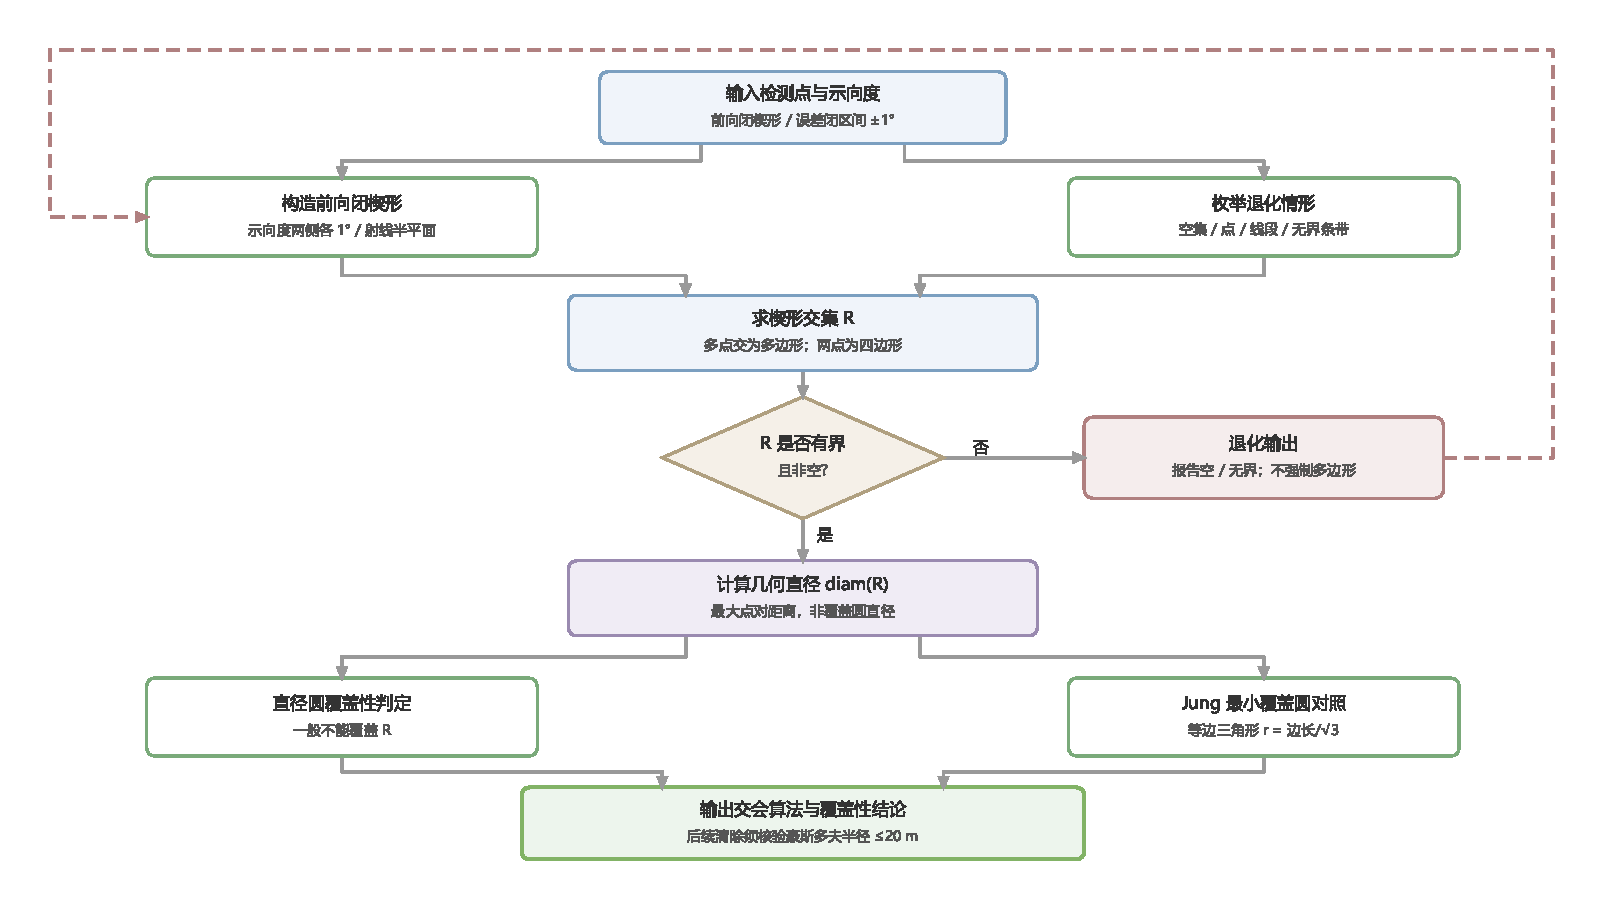
\includegraphics[width=0.82\textwidth,height=0.52\textheight,keepaspectratio]{../figures/fig_flow_q1.pdf}
\caption{问题1交会求解流程}
\label{fig:flow_q1}
\end{figure}

求解顺序是先判定线性不等式组是否可行，再判定是否在某个方向无界。
然后枚举半平面两两交点中满足全部不等式的顶点。
最后在顶点上求最远对与最小包围圆。
流程中的分支对应空集、无界、退化与多边形四类输出，避免把无界楔的直径写成一个有限数字。
实现上线性规划使用高精度单纯形，状态码为无界即判定无界，而不是用一个很大的盒子把无界截断成有限直径。
若输入示向度自相矛盾，可行判定失败，算法返回空集而不是强行给出交点。

\subsection{可行性、无界性与顶点枚举}

二维线性规划
\begin{equation}
\min\; 0^\top x\quad\mathrm{s.t.}\quad Ax\le b
\end{equation}
若无可行点，则 $R=\varnothing$，直径约定为未定义。若对某个方向 $c$ 有 $\sup\{c^\top x:x\in R\}=+\infty$，则 $R$ 无界。实现上对 $\pm e_1$、$\pm e_2$ 以及楔形角平分方向做有限次探测：线性规划状态码为无界即判定无界。无界时直径为 $+\infty$，以任何有限直径所作的圆都不能覆盖 $R$。单点检测给出的就是无界楔：两条射线之间的角域在远离检测点的方向上没有对侧约束。两点检测若夹角过小或基线与示向几乎共线，仍可能留下条带。

当 $R$ 有界时，二维凸多面体的顶点必是某两条不同约束直线的交点。对所有约束对求解 $2\times 2$ 线性方程组，丢弃平行或数值奇异的对，保留满足 $Ax\le b+\tau$ 的交点（$\tau=10^{-8}$）。所得点集去重后即顶点集 $V(R)$。三点以上时用凸包去掉内点，但直径计算并不依赖凸包：内点不可能成为最远对的端点。约束条数为 $2m$（$m$ 个检测点），顶点枚举是 $O(m^2)$ 的直线求交再过滤，竞赛尺度下 $m$ 通常不超过数十，暴力足够。后问累计裁剪时改为保留顶点循环顺序，避免每裁一条边都重建凸包，那是实现加速，不改变问题1的几何定义。

\subsection{直径算法}

凸集直径等于顶点最远对。对 $V(R)=\{v_1,\ldots,v_m\}$ 枚举
\begin{equation}
\mathrm{diam}(R)=\max_{1\le i<j\le m}\|v_i-v_j\|.
\end{equation}
$m$ 通常很小：两点交会至多四个顶点，多点交会每增加一个楔形至多增加两条边。暴力枚举对问题1足够，且避免把旋转卡壳写进必须处理退化的竞赛代码。单点时直径为 $0$；两点时直径即线段长。最远对给出的是集合的宽度上界，它回答“定位区有多大”，并不自动给出一个能盖住整个 $R$ 的圆。

同一套顶点还可用于最小包围圆。Welzl 型随机增量给出圆心 $c_\ast$ 与半径 $\rho_\ast$，满足 $R\subset \overline{B}(c_\ast,\rho_\ast)$，且 $\rho_\ast$ 最小。对三角形，若最小包围圆由最长边确定，则 $\rho_\ast=\mathrm{diam}(R)/2$；若由三顶点确定，则 $\rho_\ast>\mathrm{diam}(R)/2$。后一情形正是“直径圆不能覆盖”的几何来源。Jung 定理进一步给出平面集最小覆盖圆半径的上界 $\mathrm{diam}(R)/\sqrt{3}$；等边三角形取到该量级。因此直径、直径圆半径与 Jung 半径是三个不同对象：
\begin{equation}
\frac{\mathrm{diam}(R)}{2}\le\rho_\ast\le\frac{\mathrm{diam}(R)}{\sqrt{3}}.
\end{equation}
光学清除的充分条件是存在圆心使 $\rho_\ast\le 20$，不能用 $\mathrm{diam}(R)\le 40$ 代替。
等边三角形取到 Jung 上界量级：边长为 $1$ 时 $\rho_\ast\approx 0.5773502691948129$，与 $1/\sqrt{3}$ 一致，而直径之半为 $0.5$，严格更小。
两点楔形演示则几乎取到下界：直径 $9.877085164818205$ 的一半与包围半径 $4.938542582409102$ 在浮点精度内重合。
因此后问若用定位区选清除点，必须计算包围半径或改用边长 $28\,\mathrm{m}$ 的方格，而不能在直径小于 $40\,\mathrm{m}$ 时宣称已经可清。

\subsection{直径圆一般不能覆盖定位区域}

设 $D$ 为某条直径，以 $D$ 为直径的圆记作 $\Gamma(D)$。若 $R$ 有一个顶点不在 $\Gamma(D)$ 上，则 $\Gamma(D)$ 不能覆盖 $R$。等边三角形是标准反例：三边等长，任取一边为直径，第三顶点到该边中点的距离为边长的 $\sqrt{3}/2$，大于半径（边长之半）。因此“以直径为直径的圆”与“最小覆盖圆”不是同一对象。该反例同时回答题面“能否覆盖”：一般不能，必须按顶点几何判定，而不是写死某一个布尔值。

演示数据取边长为 $1$ 的等边三角形，算得直径 $1.0000000000134766$，最小包围圆半径 $0.5773502691948129$，直径圆覆盖判定为否。浮点残差来自坐标开方，第三顶点纵坐标为 $\sqrt{3}/2\approx 0.8660254038$，不改变判定。两点楔形交会的另一组演示给出四边形，直径 $9.877085164818205$，最小包围圆半径 $4.938542582409102$，圆心约 $(0.06095,0.06095)$，此时直径圆恰好由最长对角线生成，覆盖成立，因为 $2\rho_\ast$ 与直径在浮点精度内重合。两种情形并列，说明覆盖性不是恒真也不是恒假。

\begin{figure}[H]
\centering
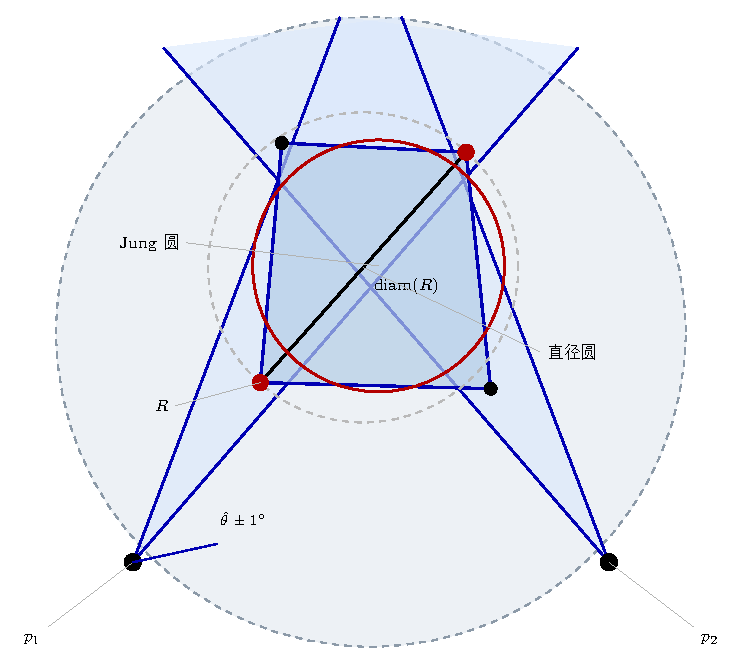
\includegraphics[width=0.82\textwidth,keepaspectratio]{../figures/tikz_wedge_q1.pdf}
\caption{楔形交会与覆盖圆}
\label{fig:tikz_wedge_q1}
\end{figure}

闭楔形交成的有界多边形落在两条示向度射线之间。
顶点最远对给出直径，Jung 圆给出真正的覆盖半径。
示意图把直径圆与 Jung 圆画在同一组顶点上，用以对照后文数值。
当三个顶点都落在最长边的直径圆上时，两圆重合；当第三顶点张成锐角等边结构时，Jung 圆必须外移。
若只看直径，会把需要三顶点定圆的情形误判为已经可被直径圆盖住。
该对照也解释了后问光学清除为什么检查包围半径而不是直径之半：等边形状的定位区会在角点留下死角，死角到直径中点的距离是边长的 $\sqrt{3}/2$，不是边长之半。

\begin{figure}[H]
\centering
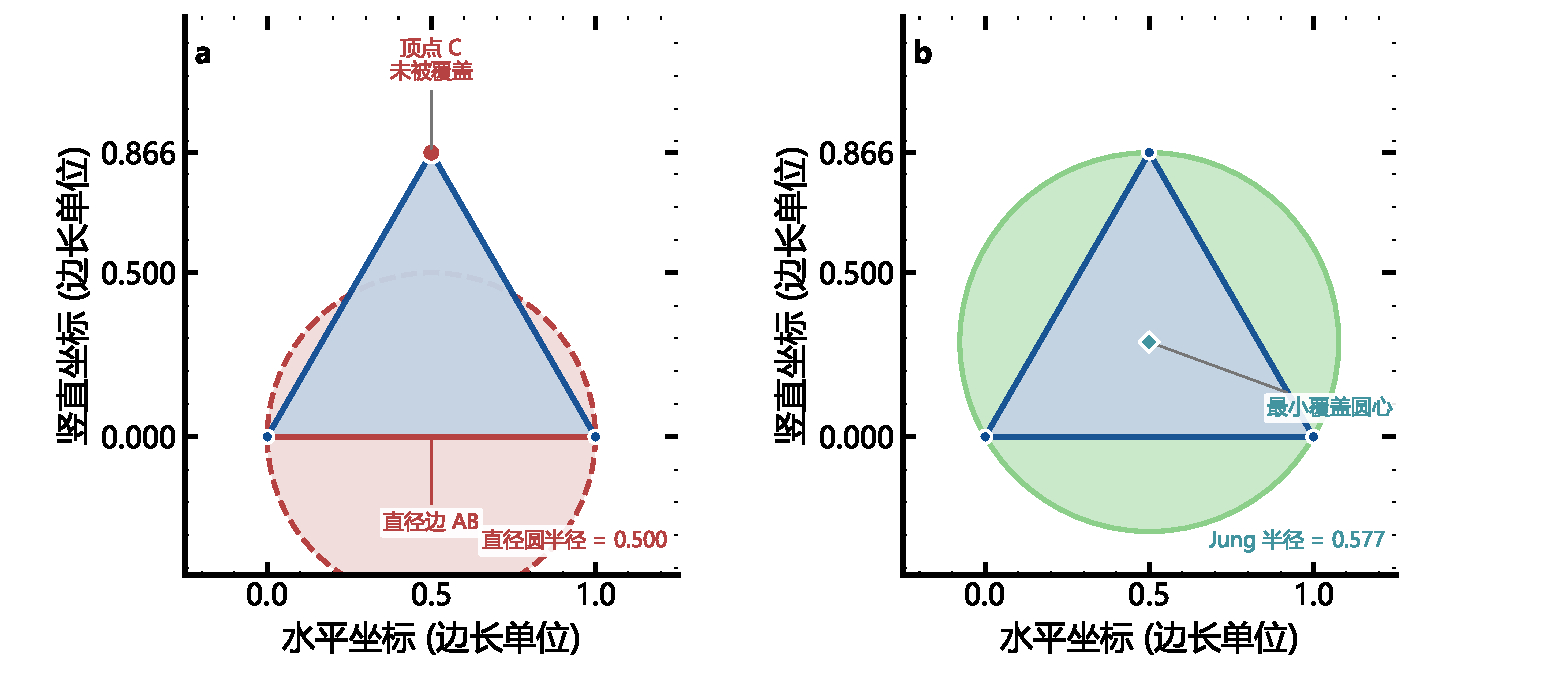
\includegraphics[width=0.92\textwidth]{../figures/fig_q1_diameter.pdf}
\caption{直径圆不能覆盖的反例}
\label{fig:q1_diameter}
\end{figure}

左面板把等边三角形的最长边作成直径圆，第三顶点落在圆外。
右面板给出 Jung 圆，半径约为边长的 $1/\sqrt{3}$。
数值上边长为 $1$ 时 $\rho_\ast\approx 0.5773502691948129$，与 $\sqrt{3}/3$ 一致，直径为 $1.0000000000134766$，覆盖判定为否。
若把 $\mathrm{diam}(R)/2$ 误当成光学清除半径，等边形状的定位区会留下角点死角。
后续选清除点时，正确的充分条件是存在圆心使包围半径不超过 $20\,\mathrm{m}$，或者用边长 $28\,\mathrm{m}$ 的方格把连续区域盖住，而不是检查直径是否小于 $40\,\mathrm{m}$。
问题1本身并不做清除，但这一几何错误若带到问题3、问题4，会在后验多边形尚未收缩到 $20\,\mathrm{m}$ 时过早宣称已经可以光学清除。
两点楔形演示给出直径 $9.877085164818205$、包围半径 $4.938542582409102$，此时直径圆恰好覆盖，说明判定随顶点集合切换，而不是写死某一个布尔值。

\subsection{与后问的衔接}

问题1交付的是一般算法，而不是某一组检测点的数字。
首先用半平面交给出凸集 $R$；再判定空集与无界；接着枚举顶点求直径与最小包围圆；最后用等边三角形与两点四边形两个演示说明覆盖性必须按几何判定。
后文问题2在单次示向度外包络上调用同一套半平面交与最小包围圆。
问题3、问题4在累计多次 $\mathtt{direction}$ 后，把新的楔形裁进已有凸多边形，直径与包围半径随观测更新。
数值上为容纳两位小数量化，后问允许把楔形半宽写成 $1.005^\circ$，但问题1按题面作答时仍用 $1^\circ$。
该包络不写入参数表，物理误差常数仍为题设的 $1^\circ$。
空集、单点、无界楔在实现里各有返回状态；开发脚本未把无界情形写进演示数据，正文不以虚构数字补全。

实现上半平面法向量由示向度方向旋转得到，不等式方向指向楔内，避免把后向角域误当成可行域。
两位小数的示向度在问题1演示中按读数使用，不额外加包络。
最小包围圆与最远对共用同一顶点集，因此直径圆能否覆盖的判定与直径计算不会各用一套点。
若输入示向度自相矛盾，线性规划无可行点，算法返回空集而不是强行给出交点。
这些分支保证后问累计裁剪时，一旦新楔形与已有多边形不相交，状态会被显式标成空，而不是留下一个过时的旧多边形继续试清。

把问题1的输出写成接口，后问才能引用而不改定义。
输入是有限个检测点及其示向度；输出是状态、顶点集、直径、最小包围圆圆心与半径、以及直径圆是否覆盖。
覆盖判定只对有界非空情形有定义：无界时任何有限圆都不能覆盖，空集时直径未定义。
等边演示把覆盖判定钉在否：直径 $1.0000000000134766$，Jung 半径 $0.5773502691948129$，第三顶点到直径中点的距离为 $\sqrt{3}/2>1/2$。
两点四边形演示把覆盖判定钉在是：直径 $9.877085164818205$，包围半径 $4.938542582409102$，圆心约 $(0.06095,0.06095)$，此时 $2\rho_\ast$ 与直径在浮点精度内重合。
二者必须同时保留，算法不读取圆域半径、接收半径或光学半径；那些量属于可行域与清除，不属于题面图2的交会多边形。
后问若要把 $R$ 与 $\Omega$ 或 $\overline B(s,1500)$ 相交，必须另开符号，不能把相交后的集合仍叫 $R$，否则问题1的直径会被后问的外包络偷偷改掉。
顶点过滤容差 $\tau=10^{-8}$ 只用于丢弃数值奇异的直线交点，不改变等边反例的几何判定。
约束条数为 $2m$，顶点枚举是 $O(m^2)$ 的直线求交再过滤；竞赛尺度下检测点数通常不超过数十，暴力足够，不必把旋转卡壳写进必须处理退化的竞赛代码。
